% Detaljer hur styrenheten är designad

\section{Styrenhet}

Styrenheten har till uppgift att ta kommandon från huvudenheten och producera utsignaler som motorer och servon kan förstå.

\subsection{Hårdvara}
Styrenheten består av en Atmega1284p, en tri-state-krets\cite{tristate}, två motorpar och en robotarm Trossenrobotics Reactor\cite{robotarm}. Styrenheten är ansluten till huvudenheten via samma 20-pinnars flatkabel som sensorenheten. Figur \ref{styr-oversikt} illustrerar grovt hur de är ihopkopplade. Bilaga \ref{kopplingsschema} visar mer detaljerat hur det är kopplat.

\begin{figure}[h!]
	\centering
	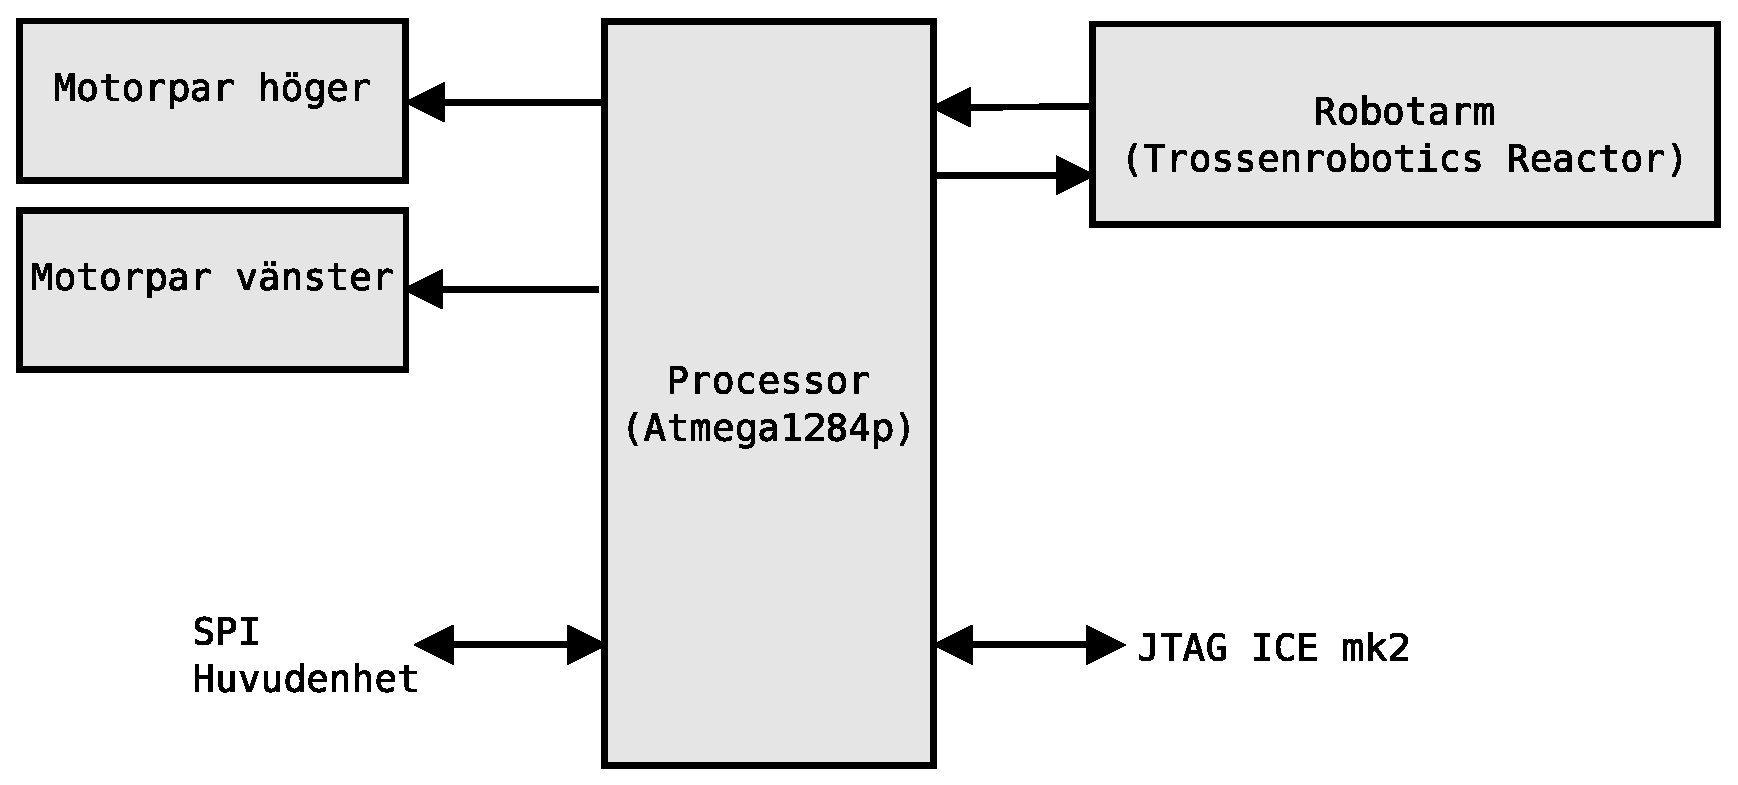
\includegraphics[scale=0.4]{grafik/styrenhet-oversikt}
	\caption{Översikt av styrenheten} \label{styr-oversikt}
\end{figure}

\subsubsection{Motorer}
Systemet har sammanlagt fyra motorer, uppdelat i två motorpar. De är anslutna till styrenheten med en 10-pinnars flatkabel. Motorparen levererades med intelligenta H-bryggor\cite{pwmmotor} och behöver förses med en PWM-signal var, som bestämmer motorernas hastighet och en riktningssignal där $1$ är i framriktningen och $0$ backriktningen.

\subsubsection{Robotarm}
Robotarmen är en Trossenrobotics Reactor och består av åtta servon av typ AX-12a\cite{servo}. Dessa är fördelade på fem axlar och en gripklo. De kommunicerar med Styrenheten över UART med en baudrate på 1MB/s, där både in och utsignal går via samma sladd. Denna är därför ansluten till två tristates för att förebygga att något oväntat skrivs eller läses från bussen.

\subsubsection{Processor}
Styrenheten drivs av en enkretsdator av typ Atmega1284p. Den kan anslutas till en PC via JTAG för att programmeras eller felsökas. Den har en klockfrekvens på 16MHz och tar emot kommandon från Huvudenheten, tolkar dessa och ser till att motorerna och robotarmen utför det som Huvudenheten har sagt. Figur \ref{styr-processor} visar hur enkretsdatorn är ansluten till övrig hårdvara.

\begin{figure}[h!]
	\centering
	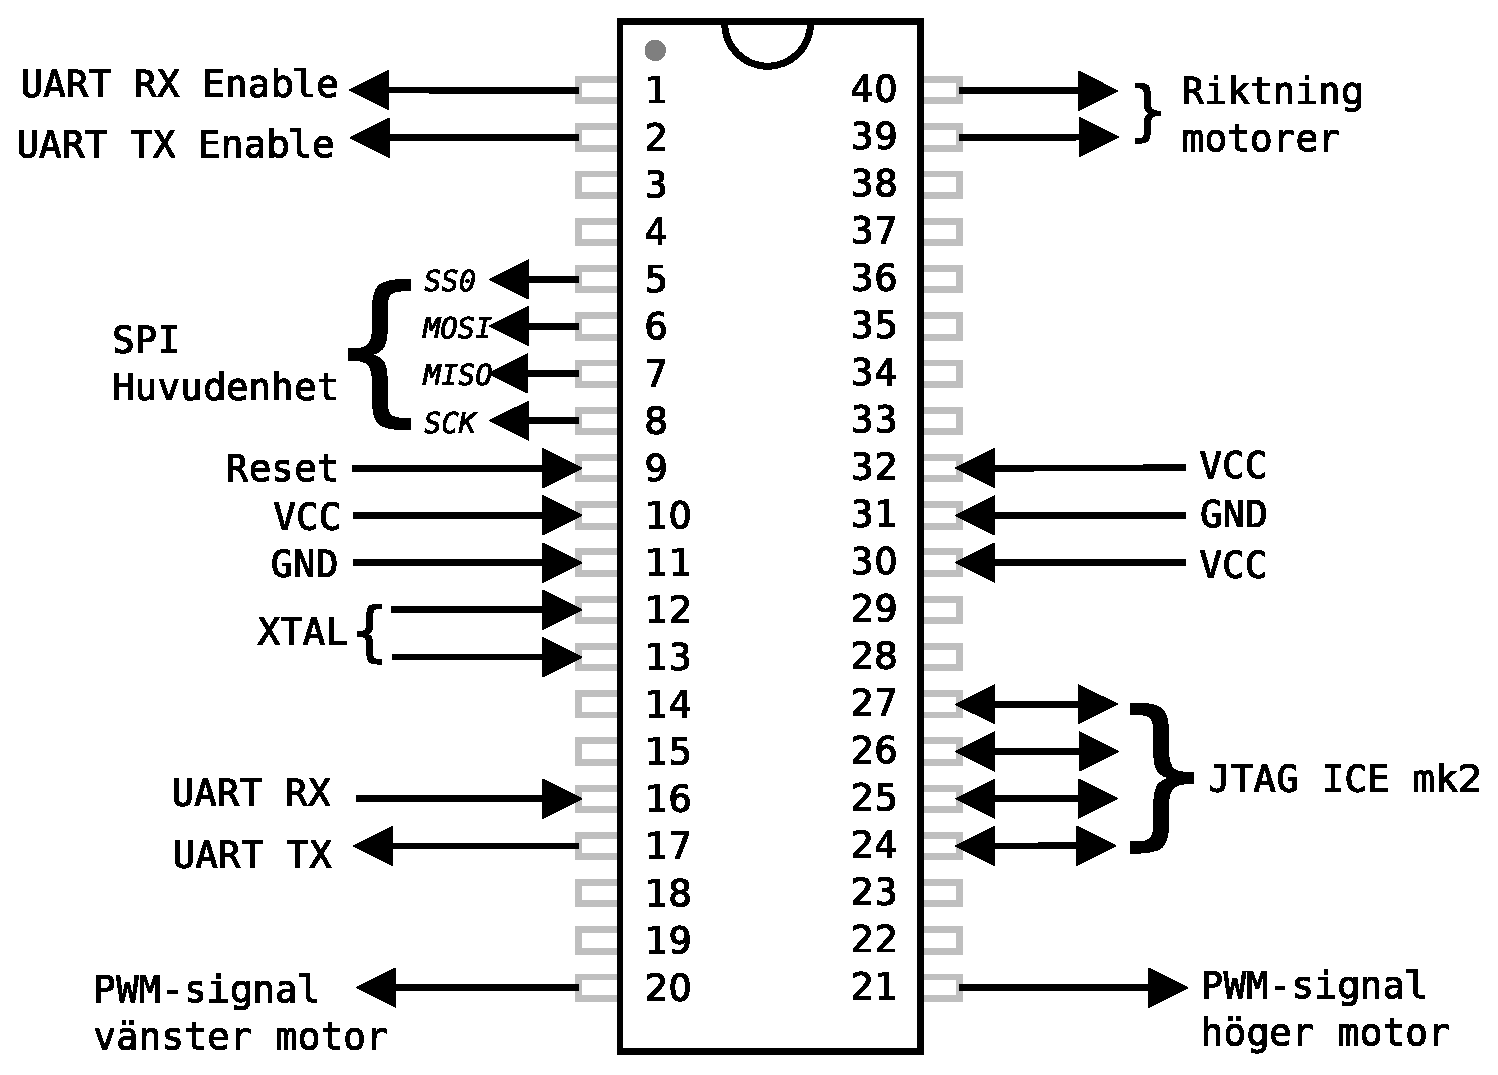
\includegraphics[scale=0.5]{grafik/styrenhet-processor}
	\caption{Schema över hur enkretssdatorn i styrenheten är ansluten till övrig hårdvara.} \label{styr-processor}
\end{figure}

\subsection{Mjukvara}
Styrenhetens mjukvara består av två moment. För det första tas kommandon emot via SPI från huvudenheten. Vi utnyttjar att Atmega1284p har hårdvarustöd för SPI och triggar ett interrupt när en byte tas emot.

\begin{figure}[h!]
	\centering
	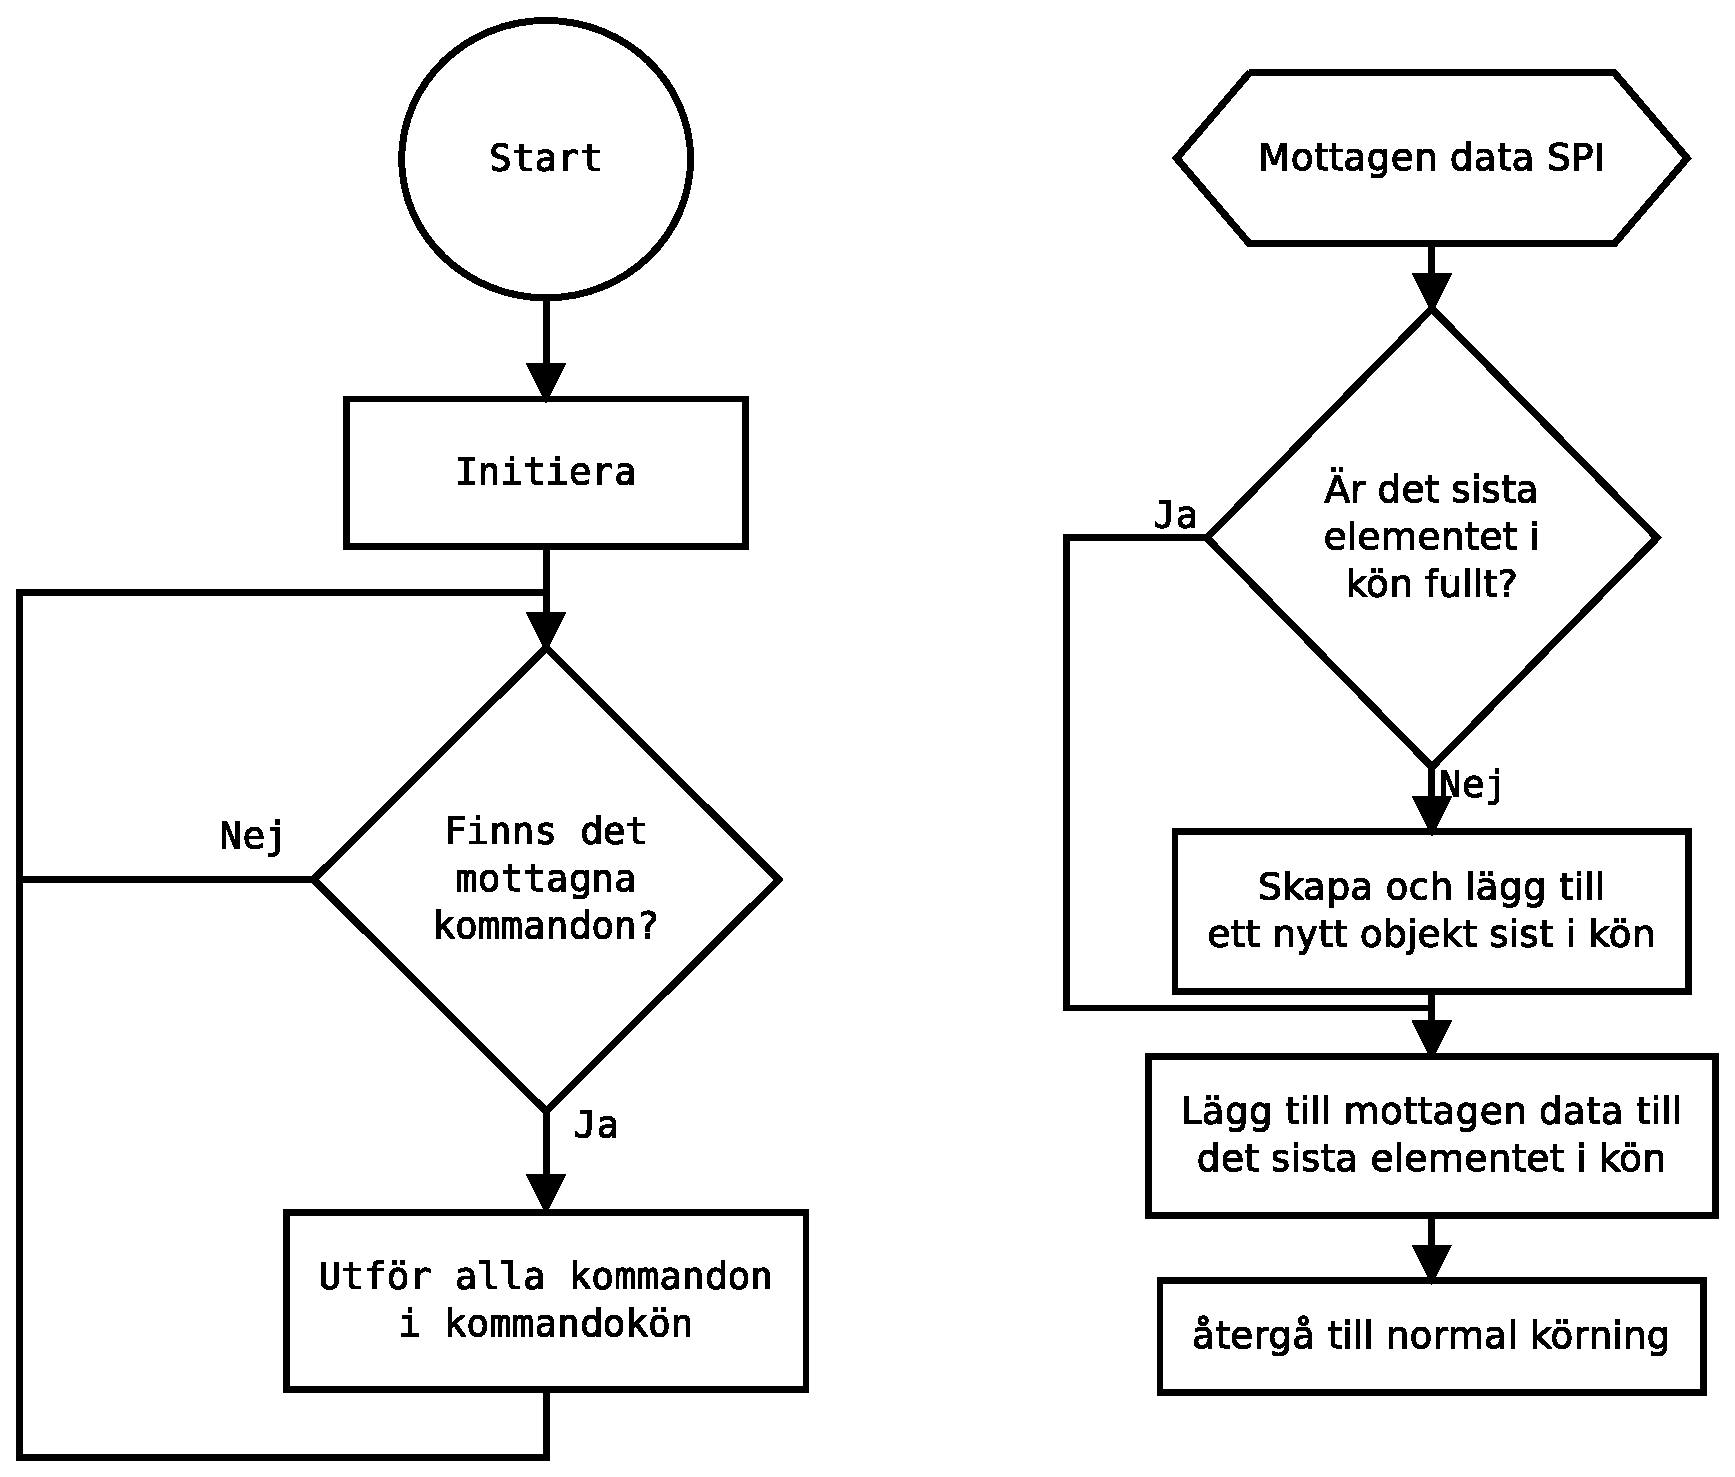
\includegraphics[scale=0.4]{grafik/styr-mjukvara}
	\caption{T.v. Styrenhetens mainloop. T.h. Hur styrenheten hanterar avbrott över SPI.} \label{styr-mjukvara}
\end{figure}

Centralt i mjukvaran är den kommandokö där mottagna databytes hamnar. Vi lägger alltid till inkomna databytes till det sista kommando-objektet i kön. Om vi får in en databyte och det sista objektet är fullt eller listan tom, skapas ett nytt kommando-objekt och läggs till kön. Vi vet att ett kommando-objekt är fullt genom att jämföra den förväntade längden (se \ref{protokoll-huvud-styr}) med hur många byte kommandot består av.

På andra sidan kommandokön har vi den del av mjukvaran som tolkar och utför inkomna kommandon. Den kollar kontinuerligt om kommandokön är tom. Är den inte det kollar vi om det första kommandoobjektet är fullt. Är det fullt mottaget tolkar vi och utför det.

Styrenheten kommunicerar med robotarmen över UART. Atmega1284p har hårdvarustöd för USART, vilket används genom att vi lägger till data till en buffert och väntar på att det skickas.

Motorernashastighet kontrolleras genom en PWM-signal till vardera motorpar. Vi utnyttjar att Atmega1284p har hårdvarustöd för två PWM-signaler som styrs av en timer var.

Styrenheten har en intern datatyp för varje enhet den förväntas styra. Om det mottagna kommandot är ett av typen \texttt{Sätt register A till D} lagras detta i den adresserade hårdvarans datatyp. I det fall att det är armen som adresseras skickas den mottagna datan till rätt register med ett \texttt{WRITE}-kommando \cite{servo}. Det innebär att armen inte realiserar de mottagna värden förrän den får ett \texttt{ACTION}-kommando. När styrenheten mottar ett \texttt{Action}-kommando från huvudenheten realiserar den tidigare mottagna kommandon för den adresserade hårdvaran. Detta görs genom att skicka \texttt{ACTION}-kommandon till armen respektive sätter de timers som styr PWM-signalerna till motorparen.
